\section{Static Analysis}
\label{sec:static-analysis}

\begin{center}
    \emph{``Success is foreseeing failure''\\}
    - Henry Petrosky
\end{center}

This section is about static analysis: what it is, how it works, what is it good for, and what are its limitations. It provides the reader with a far better understanding of static analysis, so we can further move onto the production of high quality bugs corpora, designed to assess static analysis tools.

In particular, we will focus on static analysis internals, explaining in-depth how static analyzers keep track of the control flow and data flow of the programs. We will see indeed how crucial this knowledge is when we want to inject bugs into source code in an automated way.

\subsection{Definitions}

\textbf{Static Analysis refers to any code review process performing a static examination of source code or executables, i.e., without executing it.} 

\begin{flushright}
    \emph{``The term \textbf{static analysis} refers to any process for assessing code without executing it''\\}
    \cite{chess2007secure} Brian Chess, Jacob West
\end{flushright}

The human code review process, that is to say without computer assistance is sometimes called \emph{program understanding} or \emph{program comprehension}. The term static analysis on the other hand is usually applied to the analysis performed by automated tools, also called static analyzers or static analysis tools.

Any professional who has ever written a program knows that mistakes are unavoidable, and that a systematic approach to finding bugs is compulsory. The human review of large industrial software is impractical. Therefore, automated code review should be part of any software development process.

Static analysis is useful for security, because it provides a means to perform a thorough analysis of a large code base that is not otherwise feasible. It can ``help codify best practices, catch common mistakes, and make the security process more efficient and consistent'' \cite{chess2007secure}.

\clearpage

\textbf{Static analysis tools or static analyzers are programs performing a static analysis on other programs to find security defects.}

\begin{flushright}
    \emph{``A static analyzer is a program written to analyze other programs for flaws''\\}
    \cite{black2009static} Paul E. Black
\end{flushright}

 Some static analyzers are very basic and settle for finding simple violations of programming rules or checking the improper use of vulnerable functions. But newer, sophisticated tools, go far beyond this and are capable of identifying serious problems from null-pointer de-references, buffer overflows to race conditions and other errors. They might even describe in-depth the execution trace, along with useful information about the state of the program, such as the control flow or data flow. They might as well identify values of variables leading to a failure statement \cite{anderson2008use, black2009static}.

\subsection{Strengths and Limitations of Static Analysis}

Conventionally, static and dynamic analyses are considered poles apart, because they both divide and shape the universe of methods which find security defects before they can be exploited. They have been viewed traditionally as separate domains, because they essentially use two completely opposite approaches to achieve the same goal.

Whereas static analysis operates by building a model of a program, and reasons over all the possible behaviors that might arise at run time, dynamic analysis executes the program and observes the exact run-time execution for a set of inputs \cite{ernst2003static}. Both types of analysis show their own strengths and limitations, as summarized in Table \ref{tab:static-vs-dynamic}. It is very interesting to pinpoint how static and dynamic analysis can actually work as complementary sets. One excels where the other fails, and \emph{vice versa} \cite{ernst2003static}.

Static analyses are advantageous for software security enhancement:

\begin{itemize}
    \item[\textcolor{custom-green}{\ding{51}}] By examining the code itself, and applying consistent checks, static analyzers have the capability to report the exact location in the code where a \gls{vulnerability} arises. This is really about targeting the root cause of a problem instead of its symptoms. Most of the time, static analyzers suggest mitigation recommendations, therefore reducing the research time \cite{anderson2008use,black2009static,chess2007secure}.
    \item[\textcolor{custom-green}{\ding{51}}] It is known that the longer a bug stays in the code, the more time consuming and expensive it will be to fix it. In that sense, static analyzers can be extremely powerful when properly used: they can detect \glspl{vulnerability} very early in the development lifecycle, even before the program is run for the first time. This is a huge advantage not only reducing the cost of bug fixes, but also providing the developers with a quick feedback cycle, which can help guide their work \cite{anderson2008use,black2009static,chess2007secure}.
    \item[\textcolor{custom-green}{\ding{51}}] Furthermore, as opposed to dynamic analysis, static analysis has the potential to work as a proof of correctness. This is what makes static analysis such a promising area of work: given enough time and computing power, ``static analyzers have the potential to find rare occurrences or hidden back doors. Since they consider the code independently of any particular execution, they can enumerate all possible interactions'' \cite{black2009static}. It makes it easier as well to achieve the full coverage of a large code base, because dynamic testing requires a representative set of inputs in order to perform a complete analysis on the greater number of execution paths \cite{anderson2008use,black2009static,chess2007secure,ernst2003static}.
    \item[\textcolor{custom-green}{\ding{51}}] And last but not least, new varieties of attacks are easily handled with static analysis tools. We will give an in-depth explanation about how static analyzers work in Section \ref{sub:static-analysis-internals}, but this is merely a matter of adding a rule to the tool and then rerunning it on all the code to check for the new \gls{vulnerability} \cite{anderson2008use,black2009static,chess2007secure}.
\end{itemize}

\vspace{-0.3cm}

But there are also many reasons to argue that static analysis is still limited and should never be used as a replacement for traditional dynamic analyses such as testing:

\vspace{-0.3cm}

\begin{itemize}
    \item[\textcolor{custom-red}{\ding{55}}] It is theoretically possible to design a static analyzer with the potential to be perfectly precise, by maintaining the program's full state for each and every one of the possible executions, given enough time and computing power. However, it is clear that such a tool does not exist yet \cite{anderson2008use}. In fact, it seems not feasible with the current state of the art. Modern software usually involves vast code bases composed of millions of lines of codes, with complex dependencies interactions. The number of possible executions and program states grows exponentially, withstanding even the most sophisticated analyzers \cite{anderson2008use,black2009static}.
    \item[\textcolor{custom-red}{\ding{55}}] Besides, static analyzers are limited by their inability to solve the ``Halting Problem''. ``In computability theory, the ``Halting Problem'' is the problem of determining, from a description of an arbitrary computer program and an input, whether the program will finish running or continue to run forever'' \cite{wikipedia2016halting}. In 1936, Alan Turing proved that there is no general algorithm for solving the ``Halting Problem''. That is, why recursivity and function calls made through pointers are still challenging issues for static analysis tools. Static analysis is and will remain an undecidable problem. But, in fact, this may not be the major limiting factor as long as static analysis tools are able to provide useful results \cite{anderson2008use,black2009static,chess2007secure}.
    \item[\textcolor{custom-red}{\ding{55}}] One of the most challenging tasks for analyzers is to raise their knowledge about how a program works. Making sense of a piece of code can be tedious and intricate. It involves computing and reasoning about the source code itself, what libraries a program relies on, and understanding the various and complex interactions that may occur between the different software components \cite{anderson2008use,black2009static}. ``For a static analysis tool to catch a defect, the defect must be visible in the code'' \cite{chess2007secure}. Whereas static analysis usually excels at finding violations of programming language rules, such as buffer overflows, use of deprecated functions, or common misuses of well-known libraries, it gets much more difficult for tools to report an abnormal behavior when the program does the wrong thing without crashing. Paul Anderson gives a specific example: ``if a function is intended to sort in ascending order, but perfectly sorts in descending order instead, then static analysis will not help much'' because it is ``unlikely to divine the intent of the author \dots This kind of functionality testing is what traditional dynamic testing is good for'' \cite{anderson2008use}.
    \item[\textcolor{custom-red}{\ding{55}}] Following from the above items, static analyzers atone for their limitations by making trade-offs between precision, depth, and scalability of their analyses (we will talk more about trade-offs and provide definitions of precision, depth and scalability in Section \ref{sub:diversity-of-static-analyzers}). Because of these trade-offs, static analysis tools produce \glspl{fp} and \glspl{fn}. \Glspl{fp}, also known as false alarms, are problems reported by a tool when no problem actually exists. A large number of \glspl{fp} makes it strenuous and exhausting to review an analysis report. Consequently, more important results may be overlooked. This is why \glspl{fp} are the most common complaint leveled against static analysis. Yet, when targeting security, \glspl{fn}, i.e., real problems that are not reported, are even more treacherous. Not only does your code present a vulnerability, but you live with the false sense of security that the tool did not report any flaw.
\end{itemize}

\begin{table}[ht]
    \centering
    %\rowcolors{1}{custom-light-yellow}{custom-dark-yellow}
    \begin{tabular}{p{7.8cm}p{7.8cm}}
        \toprule
        \multicolumn{1}{c}
            {\textbf{Static Analysis}} & \multicolumn{1}{c}{\textbf{Dynamic Analysis}} \\
        \midrule
            The source or binary code is analyzed \textbf{without being executed}.
        &
            The analysis is performed during the execution (\textbf{runtime analysis}) or after it using the data collected at runtime (post factum or postmortem analysis). \\
        \midrule
            \textcolor{custom-green}{$+$} No hardware and software specific to the kernel module under analysis is necessary.
        &
            \textcolor{custom-red}{$-$} If the module under analysis requires specific hardware or software, it should be provided or emulated. \\
        \midrule
            \textcolor{custom-red}{$-$} Non-trivial static analysis \textbf{requires significant amount of resources} such as time, and computing power, to be performed. This may vary according to the complexity of the analysis.
        &
            \textcolor{custom-red}{$-$} Dynamic analysis often requires fewer resources than static analysis. However, this remains a highly resource intensive process which may vary as well according to the complexity of the analysis. \\
        \midrule
            \textcolor{custom-red}{$-$} The \textbf{source code} or the binary object are \textbf{required} for analysis.
        &
            \textcolor{custom-green}{$+$} The \textbf{source code} is usually \textbf{not required} which allows to analyze software for which you do not have access to the code. \\
        \midrule
            \textcolor{custom-green}{$+$} Many (or even all) paths of execution in the code can be checked at the same time.
        &
            \textcolor{custom-red}{$-$} Only one path of execution can be checked at a time in the code. \\
        \midrule
            \textcolor{custom-green}{$+$} Static analysis has \textbf{the potential to catch every single defect in a large code base}, given enough time and computing power.
        &
            \textcolor{custom-red}{$-$} Only the \textbf{errors that occur in the path} actually executed can be detected. \\
        \midrule
            More suitable when it is enough to analyze relatively many short paths in the code (the length can be limited by "state explosion" or similar problems).
        &
            More suitable when it is necessary to analyze the execution paths in the code from the beginning to the end. \\
        \midrule
            \textcolor{custom-green}{$+$} As static analysis tools do not require the analyzed module to operate, it can be \textbf{safer} to use static analysis if it is known that the module under analysis can, for example, severely damage the system in case something goes wrong.
        &
            \textcolor{custom-red}{$-$} Dynamic analysis is sometimes less safe than static analysis because the errors in the analyzed module may have \textbf{unpredictable consequences} when the module operates. \\
        \midrule
            \textcolor{custom-red}{$-$} In many cases, static analysis is more likely to give false positives than dynamic analysis (and sometimes \textbf{the number of false positives can be unacceptable}). 
        &
            \textcolor{custom-green}{$+$} Generally, dynamic analysis tools give \textbf{less false positives} than static analysis tools (or even no false positives at all) as they usually provide the input triggering the bug. \\
        \bottomrule
    \end{tabular}
    \caption*{
        Legend:
        \begin{tabular}{ll}
             \textcolor{custom-green}{$+$} & \textcolor{custom-green}{Strength} \\
             \textcolor{custom-red}{$-$} & \textcolor{custom-red}{Limitation} \\
        \end{tabular}
    }
    \caption{Static vs. Dynamic Analysis (inspired from \cite{institute2016static})}
    \label{tab:static-vs-dynamic}
\end{table}

\clearpage

\subsection{Static Analysis Internals}
\label{sub:static-analysis-internals}

The aim of this state of the art section about static analysis is not to explain in detail all of the types of static analysis methods that exist. It gives a high level overview of how static analyzers work. Most of the examples given in this section are taken from \cite{chess2007secure} for their relevance and applicability.

The following is a high level picture of the way static analysis tools work. Regardless of the analysis techniques used, they all process source or binary code and build a model of it. The model that represents the program is analyzed according to security rules, and the tools output reports containing warnings to the user. This general process is illustrated in Figure \ref{fig:static-analysis-process} and explained in more detail throughout this section.

\vspace{0.8cm}

\begin{figure}[h]
    \centering
    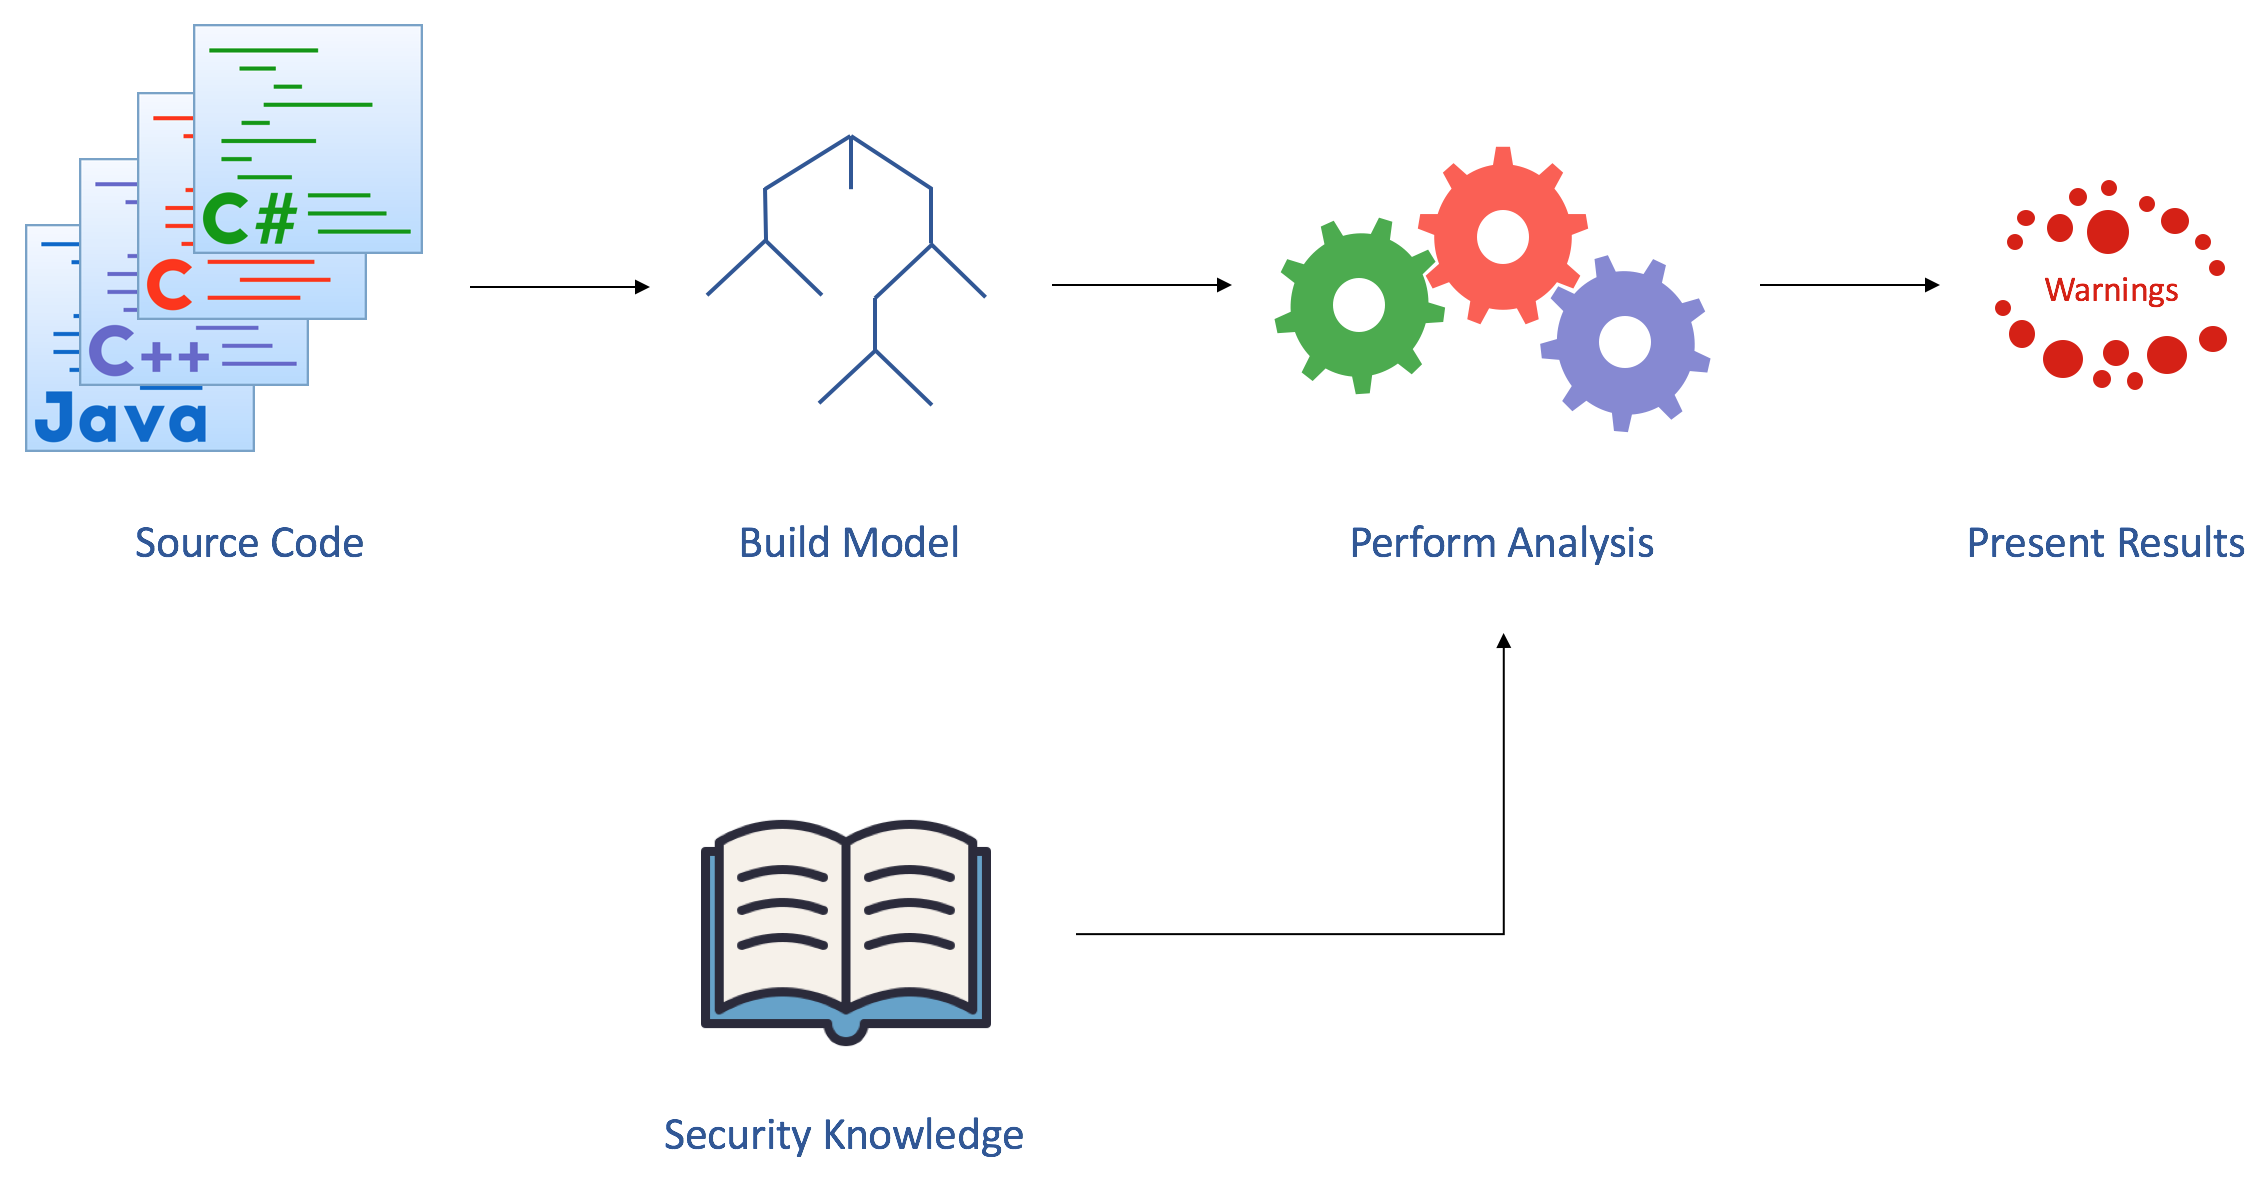
\includegraphics[scale=0.41]{figures/static-analysis-process}
    \caption{Static Analysis General Process \cite{chess2007secure}}
    \label{fig:static-analysis-process}
\end{figure}

\vspace{0.5cm}

\subsubsection{Building a Model}

It is interesting to notice than static analyzers are very similar to compilers. In fact, the first thing to do while performing a static analysis of a piece of code, is to build a model of the program. The source or binary code is transformed into a set of data structures that represent the code. To do that, static analyzers share a lot of common data structures and methods with compilers \cite{chess2007secure}.

Just like compilers, analyzers must be able to identify the source files needed to build the program. This very first step can be tricky, because source files may be scattered across many directories and mixed with superfluous code. Some sophisticated static analyzers are able to read and parse the build scripts or even observe the build system, so they retrieve important information about how a program is compiled: which compiler is being used, with which command-line flags \cite{anderson2008use}.

\clearpage

Once this first step is completed, static analyzers process the source code through three classic compilation steps:

\begin{enumerate}
    \item Lexical Analysis
    \item Syntactic Analysis
    \item Semantic Analysis
\end{enumerate}

\paragraph{Lexical Analysis}

In a nutshell, lexical analysis is the process of transforming a stream of characters into a sequence of tokens. This process, also called \emph{tokenization}, allows tools to discard the unimportant features of the program such, as whitespace or comments, and to prepare the token stream for the syntactic analysis (or simply parsing) \cite{chess2007secure,wikibooks2016compiler}.

In order to create the token stream, lexing rules are used to match the stream of characters to tokens. Tokens are also called words, and it is usual to say that tokens belong to a language. Lexical analysis rules comprise a matching table between strings of characters and words of a defined language. Regular expressions are often used to identify tokens. An example of lexing rules is given in Listing \ref{lst:lexing-rules}.

\vspace{0.5cm}

\lstinputlisting
    [
        caption=Example of Lexical Analysis Rules \cite{chess2007secure},
        label=lst:lexing-rules
    ]
    {listings/lexing-rules}

Below is a fragment of C source code:

\vspace{0.5cm}

\lstinputlisting
    [
        language=C,
        caption=A simple C program fragment \cite{chess2007secure}
    ]
    {listings/example.c}
    
If that piece of code is processed by lexical analysis according to the lexing rules in Listing \ref{lst:lexing-rules}, the stream of tokens produced would be the following:

\vspace{0.5cm}

\lstinputlisting
    [
        caption=Lexical Analysis Output \cite{chess2007secure},
        label=lst:output
    ]
    {listings/output}
    
Notice that the ID token requires the name of the identifier: this additional piece of information is later used to provide useful and precise error reporting (source line number and name of the variable). 

If the tool is just going to match the names of dangerous functions, then the job is almost finished at this point. The tool can just parse the token stream and match them with a list of deprecated, or hard to use function names \cite{chess2007secure}. For more sophisticated cases, more information is needed. The following steps provide a better understanding of the program.

\paragraph{Syntactic Analysis / Parsing}

Using the right set of words and a specific language is not enough. Should one try to make up a sentence in a foreign language, randomly putting a word after another, the probability for one to get a sentence that is grammatically correct is close to zero. Computer languages do not escape that rule.

Once the token stream is obtained, the tool needs to parse it using a grammar. A grammar is a set of production rules that matches a sequence of tokens with the correctly defined structures of a language. Listing \ref{lst:production-rules} gives an example of production rules that could be used to parse the previously obtained token stream in Listing \ref{lst:output}.

\vspace{0.5cm}

\lstinputlisting
    [
        caption=Production Rules for Parsing the Token Stream \cite{chess2007secure},
        label=lst:production-rules
    ]
    {listings/production-rules}
    
Following those production rules, the parser performs a \emph{derivation} by matching the token stream against the rules. A \emph{syntax tree} is formed in which the terminal symbols that do not carry names are omitted, so it improves the readability of the tree \cite{chess2007secure}. Applying the rules defined in Listing \ref{lst:production-rules}, one would obtain a parse tree, as shown in Figure \ref{fig:parse-tree}.

\begin{figure}[ht]
    \centering
    \begin{tikzpicture}
        \Tree   [ .stmt [ .if\_stmt
                            [ .expr [ .lval ID(ret) ] ]
                            [ .stmt
                                [ .assign\_stmt
                                    [ .lval
                                        [ .arr\_access
                                            ID(mat)
                                            [ .arr\_idx
                                                [ .expr
                                                    [ .lval ID(x) ]
                                                ]
                                            ]
                                            [ .arr\_idx
                                                [ .expr
                                                    [ .lval ID(y) ]
                                                ]
                                            ]
                                        ]
                                    ]
                                    [ .expr [ .lval ID(END\_VAL) ]
                                ]
                            ]
                        ]
                    ] 
                ]
    \end{tikzpicture}
    \caption{Syntax Tree Derived from the Sequence of Tokens \cite{chess2007secure}}
    \label{fig:parse-tree}
\end{figure}

Again, it is possible to perform some kind of static analysis at this level using the syntax tree, but it is not the best data structure to perform complex analysis. Although syntax trees are the closest representation of the code, they are derived directly from grammar production rules. Therefore it still contains superfluous nodes that makes syntax trees easy to parse and non-ambiguous. However, it also impedes the interpretation of the trees, which is the main purpose of sophisticated static analysis \cite{chess2007secure, collin2015compilation}.

For that reason, syntax trees are often re-modeled into \glspl{ast}. \glspl{ast} are simplified and standardized versions of syntax trees and offer a more natural transition to the next step: the semantic analysis of the program. Figure \ref{fig:ast} shows an AST for our example.

\begin{figure}[ht]
    \centering
    \begin{tikzpicture}
        \Tree   [ .if\_stmt
                    [ .NOT [ .COMPARE\_EQ ID(ret) 0 ] ]
                    [ .assign\_stmt
                        [ .arr\_idx
                            [ .arr\_idx ID(mat) ID(x) ]
                            ID(y)
                        ]
                        ID(END\_VAL)
                    ]
                    NO\_OP
                ]
    \end{tikzpicture}
    \caption{\acrlong{ast} \cite{chess2007secure}}
    \label{fig:ast}
\end{figure}

The simplification of the program is known as \emph{lowering}. Different levels of lowering are applied according to systems' requirements. Among possible mutations, \emph{for} loops might be converted into \emph{while} loops, or method calls could be replaced with function calls. One interesting fact is that, considering closely related programming languages, such as C and C++, one might end up with the same \glspl{ast} for the same program \cite{chess2007secure, collin2015compilation}.

However, \emph{lowering} syntax trees into \glspl{ast} has the potential effect to distort the programmer's intent. This is really important to take this into account, because we want tools to ``interpret the source code in the same way that the real compiler does'' \cite{anderson2008use}. \glspl{ast} must provide the most accurate and understandable interface, so semantic analysis can be performed optimally.

\clearpage

\paragraph{Semantic Analysis}

Once the syntactic analysis completed, the tool uses the AST to make sense of the program. The goal of syntactic analysis is to build the AST, so the tool understands how source code symbols build into language structures. Semantic analysis, on the other hand, is about attributing meaning to those structures and making sense of the program.

In order to do that, tools build a \emph{symbol table} along the \gls{ast}, as well as gathering a lot of information about the program, such as its control flow and data flow.

Briefly, the symbol table is used to give meaning to the program's symbols. It associates each identifier in the program with its type, and a pointer to its declaration or definition. This enables static analysis tools to perform some \emph{type checking} just like compilers do \cite{chess2007secure}.

From this point, static analyzers and compilers part ways. Static analyzers usually produce intermediate representations that are abstract representations of the source code, including control flow and data flow graphs, and information about the identifiers. In other words, analyzers use a high-level view of the program more suitable to their needs, going further than compilers by tracking the program's control flow and data flow. We will see how this can be achieved in the next two sections, because control flow and data flow graphs are critical parts of the model.

\subsubsection{Tracking Control Flow}

Most sophisticated static analyzers are capable of exploring the different execution paths that can possibly exist when running a program. This is made possible by tracking the control flow.

\paragraph{Control Flow Graph} Commonly, tools build a control flow graph, where nodes represent \emph{basic blocks}. Basic blocks are ``sequences of instructions that will always be executed starting at the first instruction and continuing to the last instruction, without the possibility that any instructions will be skipped'' \cite{chess2007secure}. The edges, therefore, represent the possible paths between the basic blocks.

Consider the following C code fragment shown in Listing \ref{lst:control-flow}:

\vspace{0.5cm}

\lstinputlisting
    [
        language=C,
        caption=C code fragment consisting of four basic blocks \cite{chess2007secure},
        label=lst:control-flow
    ]
    {listings/control-flow-source.c}

Figure \ref{fig:control-flow} presents the control flow graph for this C code fragment. In this example, there are only two execution paths possible or \emph{traces} through the code. ``A \emph{trace} is a sequence of basic blocks that define a path through the code'' \cite{chess2007secure}.

\clearpage

\begin{figure}[ht]
    \centering
    \begin{tikzpicture}
        % Define style
        [
            ->,
            >=stealth,
            basic-block/.style =
            {
                rectangle,
                draw=black,
                minimum height = 3em,
                inner sep = 10pt,
                text centered
            }
        ]
        % Draw nodes
        \node[  basic-block
            ] (1)
            { if (a > b) };
        \node[  basic-block,
                below left=of 1
            ] (2)
            { nConsec = 0; };
        \node[  basic-block,
                below right=of 1
            ] (3)
            {
                \begin{tabular}{l}
                    s1 = getHexChar(a);\\
                    s2 = getHexChar(b);
                \end{tabular}
            };
        \node[  basic-block,
                node distance=3.5cm,
                below=of 1
            ] (4)
            { return nConsec; };
        % Draw edges
        \path   (1) edge    node    {}  (2)
                (1) edge    node    {}  (3)
                (2) edge    node    {}  (4)
                (3) edge    node    {}  (4);
    \end{tikzpicture}
    \caption{Control Flow Graph with four basic blocks \cite{chess2007secure}}
    \label{fig:control-flow}
\end{figure}

\paragraph{Call Graph} Besides control flow graphs, tools also build \emph{call graphs} which represents the potential control flow between functions or methods. In most cases, building a call graph is quite simple. It tracks the function identifiers referenced in each function. In contrast to control flow graphs, the nodes of a call graph represent the functions, whereas the edges represent the possibility for a function to be invoked by another. Figure \ref{fig:call-graph} illustrates the call graph obtained for the C code fragment displayed in Listing \ref{lst:call-graph}.

\vspace{0.5cm}

\lstinputlisting
    [
        language=C,
        caption=C code fragment consisting of three functions definitions \cite{chess2007secure},
        label=lst:call-graph
    ]
    {listings/call-graph-source.c}

Although building a call graph seems easy, function pointers or virtual methods adds some challenges to the task. If the program dynamically loads modules at run-time, it is impossible to assess the control flow graph. In fact, tools need a combination of dataflow analysis and data type analysis to deal with it.

\clearpage
    
\begin{figure}[ht]
    \centering
    \begin{tikzpicture}
        % Define style
        [
            ->,
            >=stealth,
            function/.style =
            {
                circle,
                draw=black,
                minimum height = 4em,
                minimum width = 4em
            }
        ]
        % Draw nodes
        \node[  function
            ] (1)
            { larry };
        \node[  function,
            below right=of 1
            ] (2)
            { moe };
        \node[  function,
            below left=of 2
            ] (3)
            { curly };
        % Draw edges
        \path   (1)                 edge    node    {}  (2)
                (1)                 edge    node    {}  (3)
                (2)                 edge    node    {}  (3)
                (2) [loop right]    edge    node    {}  (2);

    \end{tikzpicture}
    \caption{Call Graph for the program in Listing \ref{lst:call-graph} \cite{chess2007secure}}
    \label{fig:call-graph}
\end{figure}

\subsubsection{Tracking Dataflow}

Sophisticated analyzers are capable of tracking the way data flows through a program. Using complex dataflow analysis algorithms, static analysis tools examine the source code and look for the locations where data is generated or used and for what purpose.

\paragraph{\gls{ssa}}

Among the dataflow analysis techniques, converting functions to their \gls{ssa} forms is very useful to keep track of where data comes from. When \gls{ssa} is applied, functions are allowed to assign a value to a variable only once in their bodies. The \gls{ssa} form makes it possible for any given value to determine easily where its value comes from \cite{chess2007secure}.

Consider the following C code fragment. Listing \ref{lst:with-ssa} presents what would be its \gls{ssa} form:

\vspace{0.5cm}

\lstinputlisting
    [
        language=C,
        caption=C code fragment in its regular form \cite{chess2007secure},
        label=lst:without-ssa
    ]
    {listings/without-ssa.c}

\vspace{0.5cm}

\lstinputlisting
    [
        language=C,
        caption=C code fragment in its \gls{ssa} form \cite{chess2007secure},
        label=lst:with-ssa
    ]
    {listings/with-ssa.c}

Transforming source code into its \gls{ssa} form can also be derived for other applications, such as finding security problems related to hard-coded values, and finding hidden backdoors. By replacing all of the instances of an \gls{ssa} variable that has been assigned a constant value by its value, you can identify defects in the code related to hard-coded values: this technique is known as \gls{cp}.

\paragraph{Taint Propagation}

Another milestone method for dataflow analysis is \gls{tp}. \Gls{tp} is about determining which data an attacker can control by analyzing the dataflow of a program. Knowing which untrusted data can be potentially used by attackers to exploit a vulnerability is a huge step towards compelling static analysis. \Gls{tp} is a key tool for identifying many input validation and representation defects \cite{chess2007secure}.

Typically, taint propagation is performed by adding labels to user-controlled data (or tainted data). Through the program, tainted data will be used to compute the values of other variables that will subsequently become tainted themselves, and so on and so forth. Thanks to this process, it is possible to track how changes in the input can affect variables much later in the program.

\Gls{tp} will be discussed in more detail later on. Even if it is possible to perform \gls{tp} statically, we will see that dynamic \gls{tp} is usually preferred. In particular, \gls{tp} is very helpful for vulnerability addition tools, such as \acrshort{lava} \cite{dolan2016lava}. Section \ref{sec:introduction-of-vulnerabilities-to-code} provides more information about \gls{lava}.

\subsubsection{Performing the Analysis - Common Algorithms}

Once the model of the program has been created, various techniques exist to analyze it. Brian Chess and Jacob West argue that ``any advanced analysis strategy consists of at least two major pieces: an \emph{intraprocedural analysis} component for analyzing an individual function, and an \emph{interprocedural analysis} component for analyzing interaction between functions'' \cite{chess2007secure}. Once again, it all comes down to the ability of static analyzers to make sense of a program. For some kinds of defects, it may be unnecessary to take the whole calling context into consideration, whereas some kind of more complex bugs would involve the code from several modules.

\paragraph{Global Analysis} Global or interprocedural analysis, as a context-sensitive analysis, is much more difficult to set up than local or intraprocedural analysis. It would be ideal if tools could perform their analysis on every function with a perfect and complete understanding of the context and environment of its calling functions. Yet, no such tool exists as global analysis definitely requires both a lot of computing power (memory) and time. The state explosion was aforementioned as one of the limititations of static analysis. Beside solutions like \emph{function summaries}\footnote{~Function summaries are basically data structures designed to hold onto precious context information such as the preconditions that the calling context must meet, and the postconditions, i.e., the effects that a function has on the run-time context when it returns}, the current state of the art is still unassertive facing that challenge.

\paragraph{Local Analysis} On the other hand, local analysis also brings its share of challenges. Nowadays, most static analyzers perform a \gls{se} on the model built during compilation, which can be seen as the simulation of an execution. Rather than using real values like a real execution would do, a \gls{se} uses abstract values, which enables property proofs while remaining a \emph{path-sensitive} analysis. \Gls{se} is based on two methods:

\begin{itemize}
    \item \Gls{ai}
    \item \Gls{mc}
\end{itemize}

\Gls{ai} refers to the process of abstracting away properties of the program that are not relevant for the analysis in place. Recursion or loops present a challenge as previously mentioned. \Gls{ai} can help avoid these problems by performing a \emph{flow-insensitive} analysis. Consider abstracting loops by examning all the possible orders in which the loop statements might be executed. You may analyze orderings that will not possibly happen, but at least, you can be sure you considered all of them. This may raise a lot of \glspl{fp}, yet it allows for the complete examination of a function while avoiding complex control flow analysis.

A \gls{mc} approach is appropriate for temporal safety properties, particularly when those properties can be defined as finite-state automatons. \Gls{mc} refers to the process of comparing the behavior of the program to a finite-state automaton, the model. Figure \ref{fig:finite-state-automaton} illustrates the model for the following property ``Memory should be freed only once'' \cite{chess2007secure}.

\vspace{1cm}

\begin{figure}[ht]
    \centering
    \begin{tikzpicture}[>=latex,shorten >=1pt, auto, node distance=3.5cm, semithick]
      \node[initial,state,minimum size=4em]      (S)                     {$Initial$};
      \node[state,minimum size=4em]              (q1)    [right of=S]    {$Freed$};
      \node[state,accepting,minimum size=4em]    (q2)    [right of=q1]   {$Error$};
    
    
      \path[->] (S)  edge [loop below] node {(other operations)} (S)
                 edge              node {$free(x)$} (q1)
            (q1) edge [loop below]  node {(other operations)} (S)
                 edge              node {$free(x)$} (q2);
    \end{tikzpicture}
    \caption{``Memory should be freed only once'' Finite-state Automaton \cite{chess2007secure}}
    \label{fig:finite-state-automaton}
\end{figure}

\subsection{Diversity of Static Analyzers}
\label{sub:diversity-of-static-analyzers}

Now that we know more about the general process followed by static analyzers, it is easy to understand why the number and the diversity of static analysis tools is striking. There is no single option way to perform static analysis. Some tools focus on simple things, such as matching name functions to warn the user for unsafe uses, whilst others try to perform more complex analysis involving control flow and dataflow tracking. Even for the same analysis scope, the type of analysis chosen can be different as various methods exist. The way the program model is built can actually be very different, because tools' \emph{foci} are not the same. ``Numerous tools are currently available. Tools vary in terms of features, supported languages, analysis methods and overall effectiveness'' \cite{delaitre2013massive}.

\subsubsection{Trade-Offs Between Precision, Depth, and Scalability}

Nowadays, static analysis methods entailing relentless accuracy are capable of examining tens of thousands of \glspl{sloc} at best. Beyond that range, the amount of memory and computing time are disproportionate. On the other end of the tools' spectrum, analyzers that perform simple static analysis algorithms are able to process millions of \glspl{sloc} or more. But to achieve their goals, tools must make trade-offs between depth, precision, and scalability.

``The depth of analysis a tool performs is often directly proportional to the scope of the analysis (the amount of the program that the tool examines at one time)'' \cite{chess2007secure}. Although a tool can process each line one at a time allowing a fast examination of the code, it narrows its analysis to a very limited understanding of the program. Other tools choose to analyze an entire program or an entire system. One can achieve better precision by providing better contextual information, but it requires more time and memory, limiting the analysis scope to small programs (less than ten thousand of \glspl{sloc}). In between, some static analyzers try to achieve both in-depth and precise analysis. Because scrutinizing the context of a program is resource intensive, those tools often limit their scopes to individual functions or modules.

Figure \ref{fig:trade-offs} taken from Brian Chess and Jacob West's book \cite{chess2007secure}, published in 2007, shows a distribution of some static analysis tools that were popular then. Note that this data might not be relevant now, but it is used here to illustrate the great variety of tools that exist. Note as well that Brian Chess and Jacob West are the founders of Fortify.

\vspace{0.5cm}

\begin{figure}[h]
    \centering
    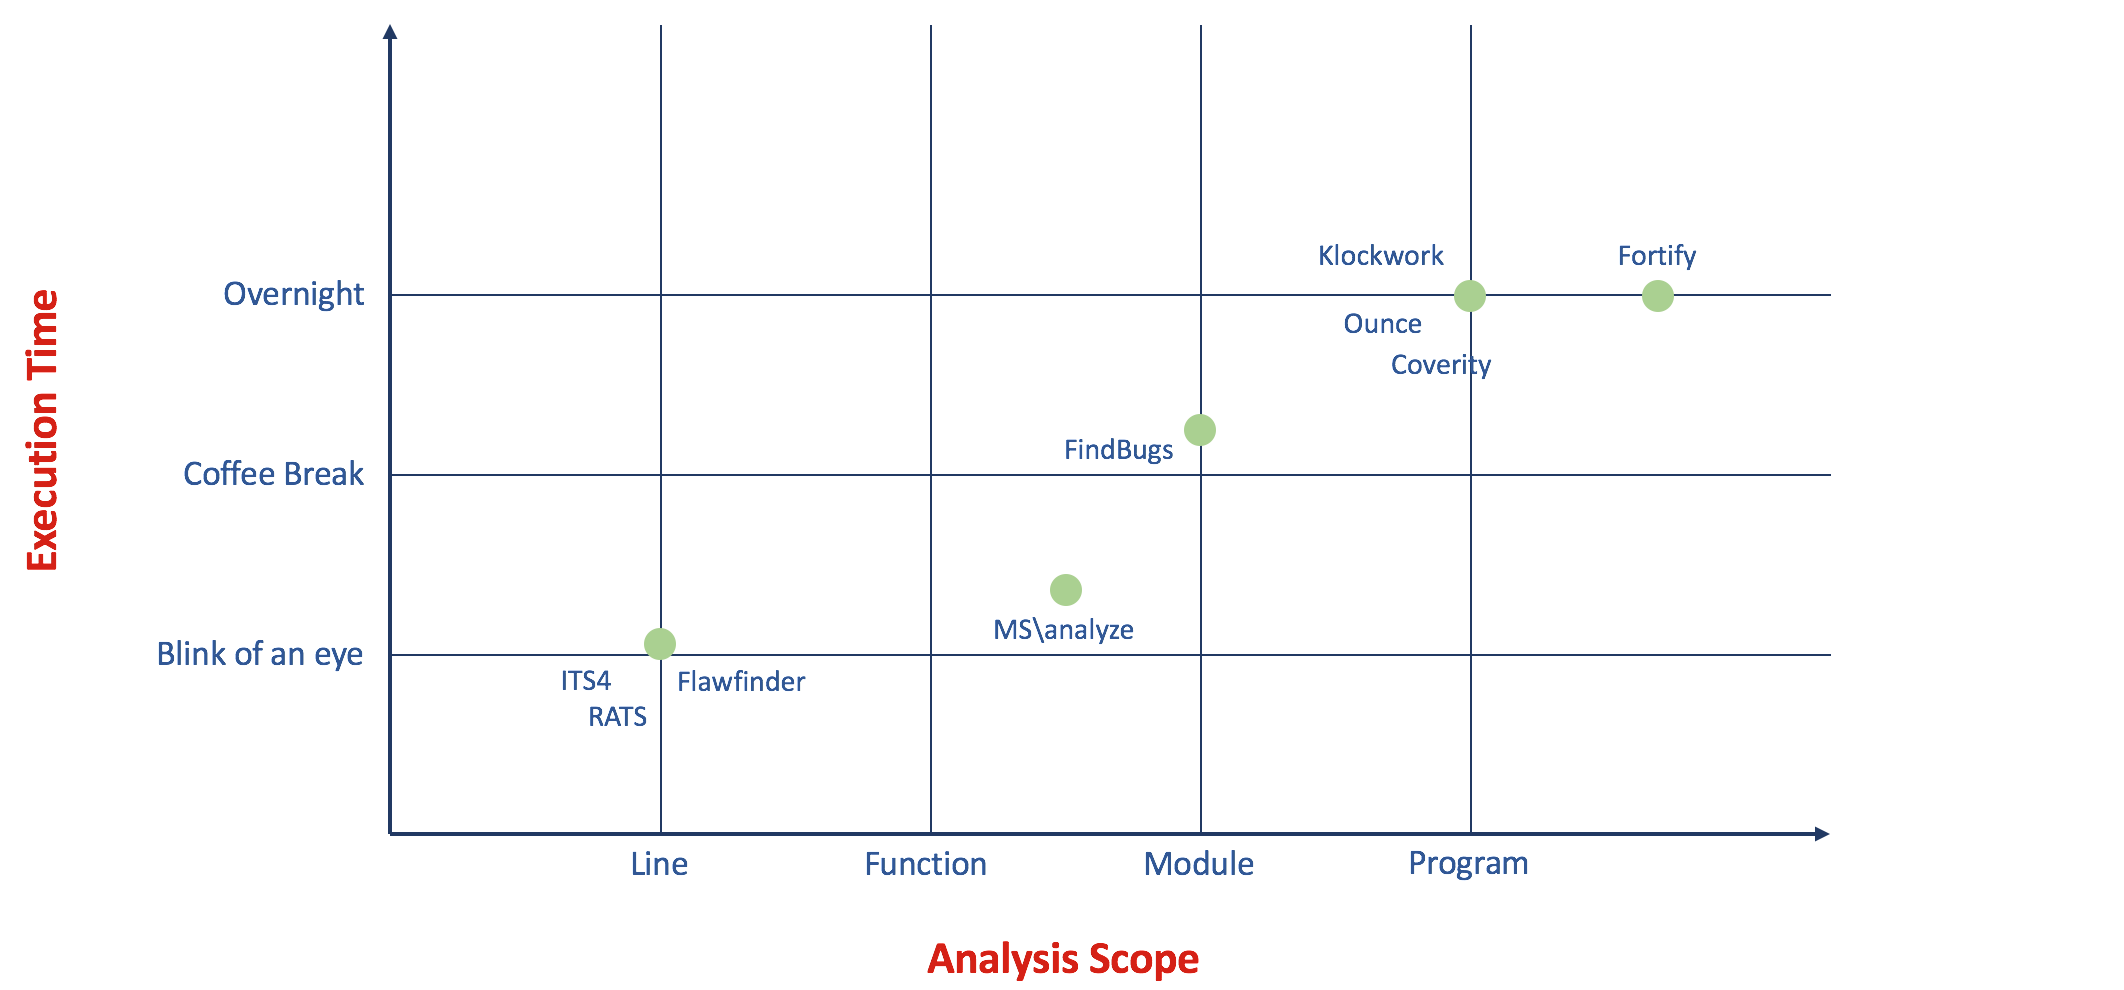
\includegraphics[scale=0.44]{figures/trade-offs}
    \caption{Analysis scope vs. Execution Time --- A Distribution of Tools \cite{chess2007secure}}
    \label{fig:trade-offs}
\end{figure}

\subsubsection{Different Features}

It is unrealistic to expect any single tool to find all types of defects. Each static analyzer is unique and provides its own set of features. In particular, static analyzers focus on specific types of vulnerabilities. Some are known to be very good at finding buffer overflows, while others may be better at finding SQL injections. But it is even more complicated than that. In fact, there are different kinds of buffer overflows, some tools may find special types of buffer overflows and not others (e.g.\ heap vs stack buffer overflows).

\subsubsection{Clarity and Ease of Use}

One factor that might be overlooked at first sight is the format of the analysis results. A tool could be the most accurate, the fastest, it does not matter if the reports provided are unclear. Keep in mind that static analyzers results are meant to be manually reviewed (software developers or security engineers most of the time). If one is not capable of interpreting the tool results, the analysis loses its value.

Reports must be complete and understandable. It should be easy as well to find the location in the code where a warning is raised. Many tools provide the user with a complete execution trace leading to the statement triggering the bug. Some even offer information about the program's dataflow. Consequently, there is no standardized way to display the analysis results: again, static analyzers handle their output in various ways.

Finally, depending on the type of analysis performed, some static analysis tools are more likely to produce a large amount of \glspl{fp}. ``Not only does wading through a long list of \glspl{fp} feel a little like serving latrine duty, but a programmer who has to look through a long list of \glspl{fp} might overlook important results that are buried in the list'' \cite{chess2007secure}. To partially overcome this issue, some tools use a system of severity to determine which warnings should first draw the reviewers' attention.

As a quick summary for this section, below can be found a small C code fragment (Listing \ref{lst:format-string-bad}) containing a format string vulnerability on line 16. Attached in Listings \ref{lst:fortify-report} and \ref{lst:frama-c-report} are the corresponding reports of Frama-C and Fortify after running on that source code.

\vfill

\lstinputlisting
    [
        language=C,
        firstline=12,
        caption=A Small Program Containing a Format String Vulnerability,
        label=lst:format-string-bad
    ]
    {listings/Format_string_problem-bad.c}
    
\vfill

\lstinputlisting
    [
        caption=Fortify Report,
        label=lst:fortify-report
    ]
    {listings/fortify-report-bad.txt}
    
\vfill
    
\lstinputlisting
    [
        caption=Frama-C Report,
        label=lst:frama-c-report
    ]
    {listings/frama-c-report-bad.txt}
    
As you can see on Listing \ref{lst:fortify-report}, Fortify provides the user with a very complete output. The line number in the source code is furnished, along with a complete trace of the execution path taken for each warning. Fortify has its own severity system as well. Classifying the warning as a format string vulnerability with high severity, not only the tool is very confident that this warning is likely to be a true positive, but it implies that the exploitability consequences of this vulnerability are critical.

On the other hand, Frama-C simply fails to find the vulnerability, and clearly provides less information than its previous challenger. However, because Frama-C seems to be less efficient than Fortify does not mean than you should use Fortify in any case. In fact, Frama-C is not really good at finding this kind of bugs. However, Frama-C is a sound tool, which means that every warning raised is correct. This property has a lot of advantages, but it limits the scalability of Frama-C. As previously mentioned, tools like Frama-C cannot process programs bigger than tens of thousands of \glspl{sloc}.